\documentclass[a4paper]{article}

%% Language and font encodings
\usepackage[english]{babel}
\usepackage[utf8x]{inputenc}
\usepackage[T1]{fontenc}

%% Sets page size and margins
\usepackage[a4paper,top=3cm,bottom=2cm,left=3cm,right=3cm,marginparwidth=1.75cm]{geometry}

%% Useful packages
\usepackage{amsmath}
\usepackage{graphicx}
\usepackage{textpos}
\usepackage{float}
\usepackage[colorinlistoftodos]{todonotes}
\usepackage[colorlinks=true, allcolors=black]{hyperref}
\usepackage[numbered,framed]{matlab-prettifier}
\usepackage{relsize}
\usepackage{amsmath}
\usepackage{amssymb}
\usepackage{amsthm}

% package to make landscape pages
\usepackage{pdflscape}

\usepackage{fancyvrb}

%% Package for graphs
\usepackage{tikz}

%% Package for loading MatLab
\usepackage[framed,numbered,autolinebreaks,useliterate]{mcode}

\setlength{\parindent}{0pt}
\newcommand{\p}{\mathbb{P}}

\title{\vspace*{2cm}17.5 Matchings\vspace*{-1.5cm}}
\date{}

\begin{document}
\maketitle

\begin{textblock*}{100mm}(0cm,-5.5cm)
\Huge 17.5
\end{textblock*}

\subsection*{Introduction}
This project will be investigating finding a 1-factor, a matching of size $n$, in a given $n \times n$ bipartite graph, or if one is not present instead finding a blocking set, a set with a neighbourhood smaller than itself.

\subsection*{Question 1}

Given an $n \times n$ bipartite graph $G$, with vertex classes $X$ and $Y$, one approach to the task of finding a 1-factor could be to check every subset $A\subseteq X$ to see if it is a blocking set. This method may be possible for small $n$ but it will soon become infeasible because it has exponential complexity, it is at least $o(2^n)$ because a given vertex class of size $n$ has $2^n$ subsets.

\subsection*{Question 2}

Let $M$ be a matching meeting the sets of vertices $A\subseteq X$ and $B\subseteq Y$. Let $u \in X\backslash A$ and let $V\subseteq Y$ consist of the vertices reachable by alternating path from $u$.

\bigskip
If $V \nsubseteq B$ then there exists $v \in V\backslash B$ with $v$ reachable from $u$ by alternating path. Let $P\subseteq E(G)$ be an alternating path from $u$ to $v$. We extend the matching $M$ to a larger matching, $M'$, between the sets of vertices $A\cup \{u\}$ and $B\cup \{v\}$ as follows (Note that $M$ and $P$ are both sets of edges so we can use set operations to determine $M'$):
\begin{align}
    \label{eq:q2}
    M' = M\backslash P + P\backslash M
\end{align}
A example to demonstrate this process on a 4x4 bipartite graph is included in figure \ref{fig:q2}.
\begin{figure}[H]
    \centering
    \begin{minipage}{0.24\textwidth}
        \centering
        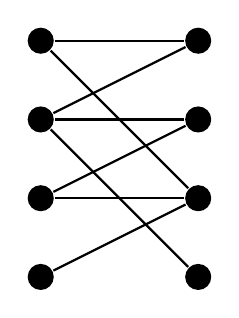
\begin{tikzpicture}
            [scale=1,auto=left,thick,every node/.style={circle,fill=black}]
            \node (A1) at (0, 0) {};
            \node (A2) at (0,-1) {};
            \node (A3) at (0,-2) {};
            \node (A4) at (0,-3) {};
            \node (B1) at (2, 0) {};
            \node (B2) at (2,-1) {};
            \node (B3) at (2,-2) {};
            \node (B4) at (2,-3) {};
            
            \draw (A1) -- (B1);
            \draw (A2) -- (B2);
            \draw (A3) -- (B3);
            \draw (A1) -- (B3);
            \draw (A2) -- (B1);
            \draw (A2) -- (B4);
            \draw (A3) -- (B2);
            \draw (A4) -- (B3);
        \end{tikzpicture}
    \end{minipage}\hfill
    \begin{minipage}{0.24\textwidth}
        \centering
        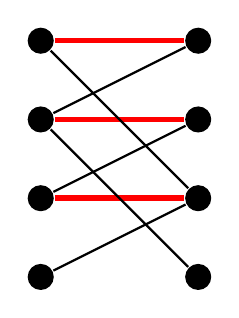
\begin{tikzpicture}
            [scale=1,auto=left,thick,every node/.style={circle,fill=black}]
            \node (A1) at (0, 0) {};
            \node (A2) at (0,-1) {};
            \node (A3) at (0,-2) {};
            \node (A4) at (0,-3) {};
            \node (B1) at (2, 0) {};
            \node (B2) at (2,-1) {};
            \node (B3) at (2,-2) {};
            \node (B4) at (2,-3) {};
            
            % matching
            \draw[line width=2pt,red] (A1) -- (B1);
            \draw[line width=2pt,red] (A2) -- (B2);
            \draw[line width=2pt,red] (A3) -- (B3);
            % rest of graph
            \draw (A1) -- (B3);
            \draw (A2) -- (B1);
            \draw (A2) -- (B4);
            \draw (A3) -- (B2);
            \draw (A4) -- (B3);
        \end{tikzpicture}
    \end{minipage}\hfill
    \begin{minipage}{0.24\textwidth}
        \centering
        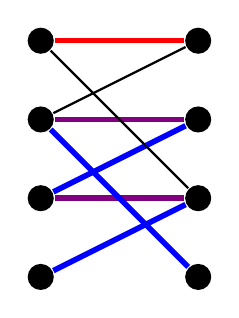
\begin{tikzpicture}
            [scale=1,auto=left,thick,every node/.style={circle,fill=black}]
            \node (A1) at (0, 0) {};
            \node (A2) at (0,-1) {};
            \node (A3) at (0,-2) {};
            \node (A4) at (0,-3) {};
            \node (B1) at (2, 0) {};
            \node (B2) at (2,-1) {};
            \node (B3) at (2,-2) {};
            \node (B4) at (2,-3) {};
            
            % matching
            \draw[line width=2pt,red] (A1) -- (B1);
            \draw[line width=2pt,red!50!blue] (A2) -- (B2);
            \draw[line width=2pt,red!50!blue] (A3) -- (B3);
            % alternating path
            \draw[line width=2pt,blue] (A4) -- (B3);
            \draw[line width=2pt,blue] (A3) -- (B2);
            \draw[line width=2pt,blue] (A2) -- (B4);
            
            % rest of graph
            \draw (A1) -- (B3);
            \draw (A2) -- (B1);
        \end{tikzpicture}
    \end{minipage}
    \begin{minipage}{0.24\textwidth}
        \centering
        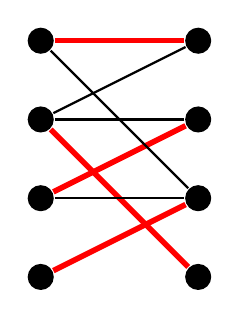
\begin{tikzpicture}
            [scale=1,auto=left,thick,every node/.style={circle,fill=black}]
            \node (A1) at (0, 0) {};
            \node (A2) at (0,-1) {};
            \node (A3) at (0,-2) {};
            \node (A4) at (0,-3) {};
            \node (B1) at (2, 0) {};
            \node (B2) at (2,-1) {};
            \node (B3) at (2,-2) {};
            \node (B4) at (2,-3) {};
            
            % matching
            \draw[line width=2pt,red] (A1) -- (B1);
            \draw[line width=2pt,red] (A4) -- (B3);
            \draw[line width=2pt,red] (A3) -- (B2);
            \draw[line width=2pt,red] (A2) -- (B4);
            
            % rest of graph
            \draw (A2) -- (B2);
            \draw (A3) -- (B3);
            \draw (A1) -- (B3);
            \draw (A2) -- (B1);
        \end{tikzpicture}
    \end{minipage}
    \caption{From left: for a small graph (black), the extension of a matching (red) via an alternating path (blue) to a larger matching (red).}
    \label{fig:q2}
\end{figure}

\subsection*{Question 3}

If $V\subseteq B$ then a blocking set can be found. Let $V'\subseteq A$ be the subset which meets $V$ according to the current matching $M$. Then $\{ u\} \cup V'$ is a blocking set. We can see this as follows.

\bigskip
Suppose $\{ u\} \cup V'$ is not a blocking set. This means its neighbourhood must be at least the same size as itself. By construction $V\subseteq \Gamma(\{ u\} \cup V')$ however it is too small to be the whole neighbourhood:
\[ |V| = |V'| < 1 + |V'| = |\{ u\} \cup V'| \]
This means there must exist an edge $xy$ with $x\in V'$, $y\in Y\backslash V$. By construction all members of $V'$ are reachable from $u$ by an alternating path, so there exists an alternating path, $P$, from $u$ to $x$. We can extend $P$ by $xy$ to produce an alternating path from $u$ to $y$. This contradicts the definition of $y$ as a vertex not in $V$ and so not reachable from $u$. Therefore we conclude that $\{ u\} \cup V'$ is a blocking set.

\subsection*{Question 4}

We now develop an algorithm to find a 1-factor by constructing successively larger matchings. Let $M$ be a matching meeting the sets of vertices $A\subseteq X$ and $B\subseteq Y$. We start with $M$ an empty matching with $A=\emptyset$ and $B=\emptyset$. The algorithm follows the steps as follows:
 \renewcommand\labelitemii{\textbullet}
\begin{itemize}
    \item
    Choose $u\in X\backslash A$ and find the set, $V$, of vertices reachable in $Y$ by an alternating path. Compare $V$ and $B$:
    \begin{itemize}
        \item
        If $V\nsubseteq B$: choose $v \in V\backslash B$ and find an alternating path, $P$, from $u$ to $v$. Use $P$ to extend $M$ according to equation \ref{eq:q2} in Question 2.
        \item
        Else $V\subseteq B$: find $V'$, the set of vertices which meet $V$ according to the matching $M$. Then $\{ u\} \cup V'$ is a blocking set and so there is not 1-factor, terminate the algorithm.
    \end{itemize}
\end{itemize}
This algorithm is very simple to implement on a bipartite graph $G$ if you are given the vertex classes of a partition as well. In the case where vertex classes are not given, to avoid having to determine a pair of vertex classes, we note that it is possible to adapt this algorithm to be as follows.

\bigskip
First check for any isolated vertices (vertices of degree 0) in $G$. If an isolated vertex is found then this is trivially a blocking set and therefore there is no 1-factor. Else there are no isolated vertices and repeat the steps as follows:
\renewcommand\labelitemii{\textbullet}
\begin{itemize}
    \item
    Consider the set of vertices $V(G)\backslash M$, that is vertices not yet included in the current matching. If this set is empty then the current matching is a 1-factor - terminate the algorithm. Else select a vertex $u\in V(G)\backslash M$ and find $V$, the set of vertices reachable from $u$ by alternating path. Compare $V$ with $V(M)$, the vertices in the current matching.
    \begin{itemize}
        \item
        If $V\backslash V(M)$ is non-empty choose a member vertex $v$ and find an alternating path $P$ from $u$ to $v$. Then extend the matching as before via $M' = M\backslash P + P\backslash M$.
        \item
        Else we have found a set of vertices, $M\cup\{u\}$, which does not contain a maximum matching and so $G$ does not contain a 1-factor. Terminate the algorithm
    \end{itemize}
\end{itemize}
We note that the first step (checking for isolated vertices) is unnecessary - the rest of the method will identify isolated vertices as blocking sets - however, we include it because it is a computationally cheap step that can save a large amount of computation in many cases.

\subsection*{Question 5}

The algorithm described in question 4 is implemented in script find\_1factor.m (pg.\pageref{Pfind_1factor}) as a function of the same name. It accepts a graph in the form of an adjacency matrix and returns a boolean indicating whether a 1-factor exists or not respectively. It then also returns the size of the blocking set if encountered, if a 1-factor is found this value is 0 indicating no blocking set found.

\bigskip
An example application of this function is included in figure \ref{fig:Q5ex}. The script correctly identifies a 1-factor in the graph from question 1.

\begin{figure}[H]
    \centering
    \begin{minipage}{0.65\textwidth}
        \centering
        \begin{verbatim}
>> G = [1,5;1,7;2,5;2,6;2,8;3,6;3,7;4,7];
>> Gmat = edgeList2adjMat(G);
>> [found, output] = find_1factor(Gmat)

found =

  logical

   1

output =

     1     5
     2     8
     3     6
     4     7
        \end{verbatim}
    \end{minipage}\hfill
    \begin{minipage}{0.35\textwidth}
        \centering
        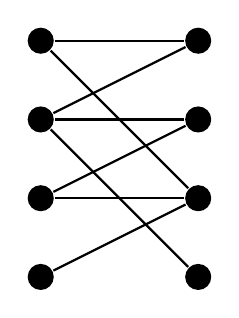
\begin{tikzpicture}
            [scale=1,auto=left,thick,every node/.style={circle,fill=black}]
            \node (A1) at (0, 0) {};
            \node (A2) at (0,-1) {};
            \node (A3) at (0,-2) {};
            \node (A4) at (0,-3) {};
            \node (B1) at (2, 0) {};
            \node (B2) at (2,-1) {};
            \node (B3) at (2,-2) {};
            \node (B4) at (2,-3) {};
            
            \draw (A1) -- (B1);
            \draw (A2) -- (B2);
            \draw (A3) -- (B3);
            \draw (A1) -- (B3);
            \draw (A2) -- (B1);
            \draw (A2) -- (B4);
            \draw (A3) -- (B2);
            \draw (A4) -- (B3);
        \end{tikzpicture}
    \end{minipage}
    \caption{An example application of find\_1factor.m to the $4\times 4$ bipartite graph from question 1.}
    \label{fig:Q5ex}
\end{figure}

\bigskip
Script Q5.m (pg.\pageref{PQ5}) applies find\_1factor.m to 20 random $n \times n$ bipartite graphs with $n=60$ for values of $p$ varying from $0.05$ to $0.35$ in steps of $0.05$ and from $0.1\ln{n}/n$ to $1.9\ln{n}/n$ in steps of $0.3\ln{n}/n$. Figures \ref{fig:q5a} and \ref{fig:q5b} include the output from Q5.m for the two ranges of $p$ respectively.

\bigskip
Inspecting the results, we see that 1-factors do not seem to appear for $p<0.9\approx 1.0\ln(40)/40$ and by $p>0.15\approx1.6\ln(40)/40$ nearly all graphs have a 1-factor. We also note that nearly all blocking sets found are trivial isolated vertices. This is likely due to the nature of the algorithm, it will find a blocking set of size 1 if present before looking for any larger blocking sets. Beyond this, however, we note that apart from blocking sets of size 1 most blocking sets are either small or large, in particular, a significant number of blocking sets are of size $n=60$. There is a symmetry in this observation because a graph cannot contain just one blocking set, take the remaining vertices and they will form a blocking set together if not multiple blocking sets. Therefore, given a large blocking set this implies the presence of a smaller blocking set elsewhere in the graph and so the observation of finding large and small blocking sets may be two observations of the same effect.

\begin{figure}[H]
    \centering
    \begin{verbatim}
p varying from 0.05 to 0.35 in steps of 0.05
ans =
  0.05        0.10        0.15        0.20        0.25        0.30        0.35  
 _______     _______     _______     _______     _______     _______     _______
 0     1     0    60     1     0     1     0     1     0     1     0     1     0
 0     1     1     0     1     0     1     0     1     0     1     0     1     0
 0     1     1     0     1     0     1     0     1     0     1     0     1     0
 0     1     0    60     1     0     1     0     1     0     1     0     1     0
 0     1     1     0     1     0     1     0     1     0     1     0     1     0
 0     1     1     0     1     0     1     0     1     0     1     0     1     0
 0     1     0    59     1     0     1     0     1     0     1     0     1     0
 0     7     1     0     1     0     1     0     1     0     1     0     1     0
 0     1     1     0     1     0     1     0     1     0     1     0     1     0
 0     3     1     0     1     0     1     0     1     0     1     0     1     0
 0     1     0     1     1     0     1     0     1     0     1     0     1     0
 0     1     0     1     1     0     1     0     1     0     1     0     1     0
 0     1     1     0     1     0     1     0     1     0     1     0     1     0
 0     1     1     0     1     0     1     0     1     0     1     0     1     0
 0     1     1     0     1     0     1     0     1     0     1     0     1     0
 0     1     1     0     1     0     1     0     1     0     1     0     1     0
 0     1     1     0     1     0     1     0     1     0     1     0     1     0
 0     1     0     1     1     0     1     0     1     0     1     0     1     0
 0     1     1     0     1     0     1     0     1     0     1     0     1     0
 0     1     1     0     1     0     1     0     1     0     1     0     1     0
    \end{verbatim}
    \caption{Output from Q5.m (column headers added) for values of $p$ varying from $0.05$ to $0.35$ in steps of $0.05$}
    \label{fig:q5a}
\end{figure}

\begin{figure}[H]
    \centering
    \begin{verbatim}
p varying from 0.1xln(n)/n to 1.9xln(n)/n in steps of 0.3xln(n)/n
ans =
   0.1         0.4         0.7         1.0         1.3         1.6         1.9    
 _______     _______     _______     _______     _______     _______     _______
 0     1     0     1     0     1     0     1     1     0     0     1     1     0
 0     1     0     1     0     1     0     1     0     1     1     0     1     0
 0     1     0     1     0     1     0    58     0    60     1     0     1     0
 0     1     0     1     0     1     0     1     1     0     1     0     1     0
 0     1     0     1     0     1     0     1     0     1     1     0     1     0
 0     1     0     1     0     1     0     1     1     0     1     0     1     0
 0     1     0     1     0     3     0    50     1     0     1     0     1     0
 0     1     0     1     0     1     0     1     1     0     1     0     1     0
 0     1     0     1     0     1     0     1     0     1     1     0     1     0
 0     1     0     1     0     1     0     1     0     1     1     0     1     0
 0     1     0     1     0     1     1     0     1     0     0     1     1     0
 0     1     0     1     0     1     0    53     0    60     1     0     1     0
 0     1     0     1     0     1     0     1     1     0     1     0     1     0
 0     1     0     1     0     1     0     1     1     0     1     0     1     0
 0     1     0     1     0     1     0     1     1     0     1     0     1     0
 0     1     0     1     0     1     0    52     1     0     0     1     1     0
 0     1     0     1     0     1     0     1     1     0     1     0     1     0
 0     1     0     1     0     1     0     1     1     0     1     0     1     0
 0     1     0     1     0     1     0     1     1     0     1     0     1     0
 0     1     0     1     0     1     0    55     1     0     1     0     1     0
    \end{verbatim}
    \caption{Output from Q5.m (column headers added) for values of $p$ varying from $0.1\ln{n}/n$ to $1.9\ln{n}/n$ in steps of $0.3\ln{n}/n$}
    \label{fig:q5b}
\end{figure}

\subsection*{Question 6}

Script Q6.m (pg.\pageref{PQ6}) runs find\_1factor.m on ten random bipartite graph processes with $n=40$. For each process the the script checks each graph in turn for a 1-factor and once a 1-factor is found we observe that all following graphs will contain this 1-factor. Figure \ref{fig:q6tab} includes a sample of the full tabulated data. Figures \ref{fig:q6summary} and \ref{fig:q6output} include further output summarising a couple of interesting points from the full data set.

\begin{figure}[H]
    \centering
    \begin{verbatim}
edges   rep_1  rep_2  rep_3  rep_4  rep_5  rep_6  rep_7  rep_8  rep_9  rep_10
_____   _____  _____  _____  _____  _____  _____  _____  _____  _____  ______
141     0   1  0  27  0   1  0   1  0   1  0   1  0   1  0   1  0   1  0   1
140     0   1  0  27  0   1  0   1  0   1  0   1  0   1  0   1  0   1  0   1
142     0   1  0  27  0   1  0   1  0   1  0   1  0   1  0   1  0   1  0   1
143     0   1  0  27  0   1  0   1  0   1  0   1  0   1  0   1  0   1  0   1
144     0   1  0  27  0   1  0   1  0   1  0   1  0   1  0   1  0   1  0   1
145     0   1  0  32  0   1  0   1  0   1  0   1  0   1  0   1  0   1  0   1
146     0   1  0  32  0   1  0   1  0   1  0   1  0   1  0   1  0   1  0   1
147     0   1  0  32  0   1  0   1  0   1  0   1  0   1  0   1  0   1  0   1
148     0   1  0  32  0   1  0   1  0   1  0   1  0   1  0   4  0   1  0   1
149     0   1  0  32  0   1  0   1  0   1  0   1  0   1  0   4  0   1  0   1
150     0   1  0  32  0   1  0   1  0   1  0   1  0   1  0   4  0   1  0   1
151     0   1  0  32  0   1  0   1  0   1  0   1  0   1  0   4  0   1  0   1
152     0   1  0  32  0   1  0   1  0   1  0   1  0   1  0   4  0   1  0   1
153     0   1  1   0  0   1  0   1  0   1  0   1  0   1  0   4  0   1  0   1
154     0   1  1   0  0   1  0   1  0   1  0   1  0   1  0   4  0   1  0   1
155     0   1  1   0  0   1  0   1  0   1  0   1  0   1  0   4  0   1  0   1
156     0   1  1   0  0   1  0   1  0   1  0   1  0   1  0   4  0   1  0   1
157     0   1  1   0  0   1  0   1  0   1  0   1  0   1  1   0  0   1  0   1
158     0   1  1   0  0   1  0   1  0   1  0   1  0   1  1   0  0   1  0   1
159     0   1  1   0  0   1  0   1  0   1  0   1  0   1  1   0  0   1  0   1
160     0   1  1   0  0   1  0   1  0   1  0   1  0   1  1   0  0   3  0   1
161     0   1  1   0  0   1  0   1  0   1  0   1  0   1  1   0  0   3  0   1
162     0   1  1   0  0   1  0   1  1   0  0   1  0   1  1   0  0   3  0   1
163     0   1  1   0  0   1  0   1  1   0  0   1  0   1  1   0  0   3  0   1
164     0   1  1   0  0   1  0   1  1   0  0   1  0   1  1   0  1   0  0   1
165     0   1  1   0  0   1  0   1  1   0  0   1  0   1  1   0  1   0  0   1
    \end{verbatim}
    \caption{Sample of tabulated data from Q6.m: For each rep the left column indicates the presence of a 1-factor and the right column records the size of the blocking set if encountered.}
    \label{fig:q6tab}
\end{figure}

\begin{figure}[H]
    \centering
    \begin{verbatim}
summary =
  10×2 table
  
    NoTrivial    first1Factor
    _________    ____________
    170          170         
    111          153         
    202          202         
    185          185         
    162          162         
    199          199         
    197          197         
    148          157         
    160          164         
    221          221        
    \end{verbatim}
    \caption{Summary of two key data points collected from Q6.m: 'NoTrivial' records the number of edges added to each random bipartite graph process before all trivial blocking sets are removed. 'first1Factor' records the number of edges added before the first 1-factor was found for each process.}
    \label{fig:q6summary}
\end{figure}

\begin{figure}[H]
    \centering
    \begin{verbatim}
Average edges before all trivial blocking sets removed:
ans =
  175.5

Average edges before 1-factor found:
ans =
   181

Reps where 1-factor found as soon as all trivial blocking sets removed
ans =
     7
    \end{verbatim}
    \caption{Some further points of interest calculated by Q6.m from the data in figure \ref{fig:q6summary}.}
    \label{fig:q6output}
\end{figure}

% \bigskip
% To improve efficiency we note that for a random bipartite process any subgraphs present in a given member of the sequence will be present in all following graphs because edges are never removed. Therefore, as soon as a matching is found in a given process then that matching will apply for all future members of the process. In a similar way we observe that a blocking set in one member of the sequence will remain a blocking set in subsequent graphs until sufficient edges are added. Therefore, with a blocking set from one graph we test whether that same blocking set remains a blocking set in the following graph to save repeating work. If it remains a blocking set then we can move on to the next graph, if not than we check for a 1-factor.

\bigskip
We note a couple simple properties of a graph necessary for a 1-factor to exist:
\begin{itemize}
    \item
    The graph must have at least as many edges as are required for a 1-factor. In the case of an $n\times n$ bipartite graph this is $n$.
    \item
    There may be no isolated vertices (vertices of degree 0).
    \item
    There may be no maximal path (a path which cannot be extended) of length two. 
\end{itemize}
% We combine these to form a stronger necessary condition: No component of the graph may have an odd size. Isolated vertices, which would otherwise form trivial blocking sets, are components of size 1 and so are not present. Further, given all vertices are degree at least 1 we have that there are at least as many edges as are required for a 1-factor.

\subsubsection*{Inspection of Results}

Looking at the data from Q6.m, figures \ref{fig:q6summary} and \ref{fig:q6output}, we see that once sufficient edges have been added in a random bipartite graph process to eliminate all isolated vertices then the graph is very likely to also have enough edges to form a 1-factor. In particular, in figure \ref{fig:q6output} we see that 7 out of 10 of the processes found a 1-factor immediately after eliminating all isolated vertices.

\subsubsection*{Sharp Threshold for Isolated Vertex}
Due to the necessity of being free of isolated vertices in order to contain a 1-factor we consider the threshold for a random bipartite graph to be free of isolated vertices. We now demonstrate that $f: n \mapsto \log{n}/n$ is a sharp threshold for $G \in \mathcal{G}(n,p)$ to have an isolated vertex.

\bigskip
Let $X$ denote the number of isolated vertices in $G$. First we calculate the expectation and variance.

\bigskip
Expectation:
\begin{align*}
    \mu = \mathbb{E}(X) = 2n(1-p)^{n}
\end{align*}
Variance: where $X = \sum_{i=1}^N A_i$ and $A_i$ denotes the event that vertex $i$ is isolated.
\begin{align*}
    Var(X) &= \sum_{i=1}^N \sum_{j=1}^N [\mathbb{P}(A_i \cap A_j) - \mathbb{P}(A_i)\mathbb{P}(A_j)] \\
    \sigma^2 &= \sum_{i=1}^{2n} \sum_{i,j \text{ diff class}} [(1-p)^{2n-1} - (1-p)^n\times(1-p)^n] \\
             &= 2n \times n \times (1-p)^{2n-1}[1 - (1-p)] \\
             &= 2n^2p(1-p)^{2n-1}
\end{align*}

\bigskip
By Markov's Inequality:
\begin{align*}
    \mathbb{P}(X\neq0) &= \mathbb{P}(X \geq 1) \leq \frac{\mathbb{E}(X)}{1} = \mu
\end{align*}
Noting the inequality:
\begin{align*}
    2n(1-p)^n < 2ne^{-pn}
\end{align*}
Then taking $p = o(\log{n}/n)$:
\begin{align*}
    \mathbb{P}(X\neq0) < o( ne^{-\frac{\log{n}}{n} n} ) = o( ne^{-\log{n}} ) = o( n\frac{1}{n} ) = o(1)
\end{align*}
Hence if $p=o(\log{n}/n)$ then almost every $G \in \mathcal{G}(n,p)$ is free of isolated vertices.

\bigskip
By Chebyshev's Inequality:
\begin{align*}
    \mathbb{P}(X=0) &\leq \mathbb{P}(|X-\mu| \geq \mu) \leq \frac{Var(X)}{\mu^2} = \frac{\sigma^2}{\mu^2}
\end{align*}
Substituting values for $\mu$ and $\sigma$:
\begin{align*}
    \frac{\sigma^2}{\mu^2} &= \frac{2n^2p(1-p)^{2n-1}}{[2n(1-p)^n]^2} = \frac{p}{2(1-p)}
\end{align*}
Taking $p = o(\log{n}/n)$:
\begin{align*}
    \frac{\sigma^2}{\mu^2} &\leq o\Bigg( \frac{\log{n}/n}{2(1-\log{n}/n)} \Bigg) \\
                           &= o\Bigg( \frac{\log{n}}{(n-\log{n})} \Bigg) \\
                           &= o\bigg( \frac{\log{n}}{n} \bigg) \\
                           &\rightarrow 0 \quad \text{as} \quad n \rightarrow \infty
\end{align*}
Hence if $p=\omega(\log{n}/n)$ then almost every $G \in \mathcal{G}(n,p)$ contains an isolated vertex.

\bigskip
Therefore we conclude that the function $f: n \mapsto \log{n}/n$ is a sharp threshold for $G \in \mathcal{G}(n,p)$ to have an isolated vertex. This may motivate the choice of $p$ varying from $0.1\ln{n}/n$ to $1.9\ln{n}/n$ given in Question 5 because this range spans well this sharp threshold and the property of being free of isolated vertex is, as mentioned previously, a necessary condition for containing a 1-factor.

\subsubsection*{Maximal paths of length 2}
Further, we now consider the presence of maximal paths of length two. In other words, these are $P_2$ subgraphs for which the end vertices are degree 1 (note that the middle vertex may have a degree greater than 2). Let $Y$ denote the number of maximal paths of length 2 in $G\in \mathcal{G}(n,p)$. We note that a random graph may have few maximal paths of length 2 because either there are insufficient edges to form any or there are too many present. We are interested in the later case. Here we show that for $p=o(1/\sqrt{n})$ then $\mathbb{P}(Y>0) \rightarrow 0$ as $n\rightarrow\infty$.

Expectation of $Y$:
\begin{align*}
    \mu = \mathbb{E}(Y) &= 2n \times {n\choose2} \times p^2(1-p)^{2(n-1)} \\
                        &= n^2(n-1)p^2(1-p)^{2n-2} \\
\end{align*}
By Markov's Inequality:
\begin{align*}
    \mathbb{P}(Y\neq0) &= \mathbb{P}(Y \geq 1) \leq \frac{\mathbb{E}(Y)}{1} = \mu
\end{align*}
Taking $p=o(1/\sqrt{n})$
\begin{align*}
    \mathbb{P}(Y\neq0) &\leq o\bigg( n^2(n-1)(\frac{1}{\sqrt{n}})^2\big(1-\frac{1}{\sqrt{n}}\big)^{2n-2} \bigg) \\
                       &\leq o\bigg( n^2\big(1-\frac{1}{\sqrt{n}}\big)^{2n} \bigg) \\
    \Rightarrow \mathbb{P}(Y\neq0) &\rightarrow 0 \qquad n\rightarrow\infty
\end{align*}
The final step follows because the latter term is exponential and so suppresses the algebraic $o(n^2)$ term. Therefore we conclude that for $p=o(1/\sqrt{n})$ we expect $G\in \mathcal{G}(n,p)$ to be free of maximal paths of length 2. This could potentially be a motivation for the choice in question 5 of $p$ varying between 0.05 and 0.35 because $1/\sqrt{n} \approx 0.158$ for $n=40$ which is spanned by this range of $p$.


\subsection*{Question 7}

We now consider the complexity of the algorithm to find a 1-factor. The implementation in find\_1factor.m is approximately order $o(n^3)$. This can be seen by considering the steps of the algorithm as follows:

\begin{enumerate}
    \item
    Checking for isolated vertices has complexity $o(n^2)$ because in the worst case of just one isolated vertex potentially the presence of all edges would be checked.
    \item
    Each iteration of the algorithm adds one edge to the matching. Therefore, finding a 1-factor requires $o(n)$ iterations.
    \item
    Determining unused vertices via an adjacency matrix requires $o(n^2)$ operations. This is because the columns must be summed and then inspected.
    \item
    Finding vertices reachable from $u$ by an alternating path is $o(n^2)$. In the worst case all members of the opposite class could be reachable but each iteration of this subroutine finds only one of those vertices at a time. Checking though all currently reachable vertices on each iteration and only finding one new vertex every loop has a complexity of $o(n^2)$.
    \item
    Finding an alternating path, given the record kept while determining reachable points, is order $o(n)$. This method simply follows the steps backwards from $v$ to $u$ and since an alternating path can be at most length $2n-1$ we have $o(n)$.
    \item
    Computing a new matching with an alternating path is $o(n)$ because there are at most $(n-1) + (2n-1)$ edges to compare in order to determine $M\backslash P$ and $P\backslash M$.
\end{enumerate}
Combining the above, we conclude that the complexity of find\_1factor.m is
\[ o(n^2) + o(n) \times \big( o(n^2) + o(n) + o(n) \big) = o(n^3) \]

\subsubsection*{Adjacency List}
Alternatively to an adjacency matrix, a graph can be described by an adjacency list. For sparse graphs this can represent a significant improvement in efficiency, not just because of the reduction in required storage.

\bigskip
Using an adjacency list would affect all the slowest, $o(n^2)$, steps (1, 3 and 4) described in the complexity summary above. This is because checking a adjacency list for edges in a sparse graph can be seen to be an $o(1)$ complexity task compared with checking an adjacency matrix for every possible edge connected to a given vertex which is $o(n)$. Completing a similar complexity calculation as before we see that overall this reduces the complexity of the algorithm to $o(n^2)$.

\subsection*{Question 8}

The alternating path method for finding a 1-factor is effective for all graphs, not just bipartite graphs. We can see this because a 1-factor is by construction bipartite. For a graph to contain a 1-factor this implies that it contains a bipartite sub-graph. Even in the worse case, for any graph we can apply the algorithm to every bipartite subgraphs until a 1-factor is found.

\bigskip
However, with further inspection we wee that the algorithm as described in my adapted algorithm in question 4 can be applied immediately to any graph. The algorithm does not require two bipartite vertex classes, all that is required is to consider vertices present and absent in the current matching. To see this we consider the following two observations:
\begin{itemize}
    \item 
    The task is in one respect symmetric: In the bipartite case, starting with the vertex classes either way round will achieve the same conclusion (not necessarily the same 1-factor/blocking set).
    \item
    The task is in one respect asymmetric: An alternating path is specially a path such that every \textbf{second} edge is in $M$. In particular, a path such that every other edge is in $M$, starting from the first edge in $M$, is not an alternating path.
\end{itemize}
This means that on each iteration we can simply choose any point not present in the current matching and seek to add it in. We don't need an explicit bipartite partition of $G$ because the alternating path definition will only permit the algorithm to find reachable vertices which are in the opposite vertex class of some valid bipartite partition of $G$.

\subsection*{Question 9}

In the case of a bipartite graph with no 1-factor the algorithm can be modified to find a maximum matching as follows. When a blocking set is found, instead of terminating the process, remove and discard from the process the vertex whose addition lead to the blocking set and then resume the process. Eventually, every vertex will either have been removed or added to the matching and the matching will be a maximum matching.

% Removing the vertex will be sufficient to remove the blocking set because of how we found the blocking sets. If we encounter a blocking set of  - their neighbourhoods are only ever one larger than themselves so the removal of just one vertex will be sufficient to stop them being blocking.

\pagebreak
\section*{Programs}

\subsection*{find\_1factor.m}\label{Pfind_1factor}
Dependencies: edgeList2adjMat.m (pg.\pageref{PedgeList2adjMat}), findReachable.m (pg.\pageref{PfindReachable}), findAltPath.m (pg.\pageref{PfindAltPath}).
\lstinputlisting{find_1factor.m}

\subsection*{edgeList2adjMat.m}\label{PedgeList2adjMat}
\lstinputlisting{edgeList2adjMat.m}

\newpage
\subsection*{findReachable.m}\label{PfindReachable}
\lstinputlisting{findReachable.m}

\subsection*{findAltPath.m}\label{PfindAltPath}
\lstinputlisting{findAltPath.m}

\newpage
\subsection*{Q5.m}\label{PQ5}
Dependencies: ranBip.m (pg.\pageref{PranBip}), find\_1factor.m (pg.\pageref{Pfind_1factor}).
\lstinputlisting{Q5.m}

\subsection*{ranBip.m}\label{PranBip}
\lstinputlisting{ranBip.m}

\newpage
\subsection*{ranBipProcess.m}\label{PranBipProcess}
\lstinputlisting{ranBipProcess.m}

\newpage
\subsection*{Q6.m}\label{PQ6}
Dependencies: ranBipProcess.m (pg.\pageref{PranBipProcess}), find\_1factor.m (pg.\pageref{Pfind_1factor}).
\lstinputlisting{Q6.m}

\end{document}
